% create the angle used to reduce SO2 symmetry of two states which
% are related by reflection
% use package tikz
% By Xiong
% 
% use the following command to generate the pdf
% pdflatex --jobname=C3orbits-f1 C3orbits.tex

\documentclass{article}
\usepackage{graphicx}
\usepackage{tikz}
\usetikzlibrary{calc}
\usetikzlibrary{arrows}
\usetikzlibrary{decorations.markings}
\usetikzlibrary{decorations.pathreplacing}

\tikzset{
  big arrow/.style={
    decoration={markings,mark=at position 0.5 with {\arrow[scale=1.5,blue]{#1}}},
    postaction={decorate},
    shorten >=0.4pt},
  big arrow/.default=>
}

\pgfrealjobname{C3orbits}


\begin{document}

\beginpgfgraphicnamed{C3orbits-f1}
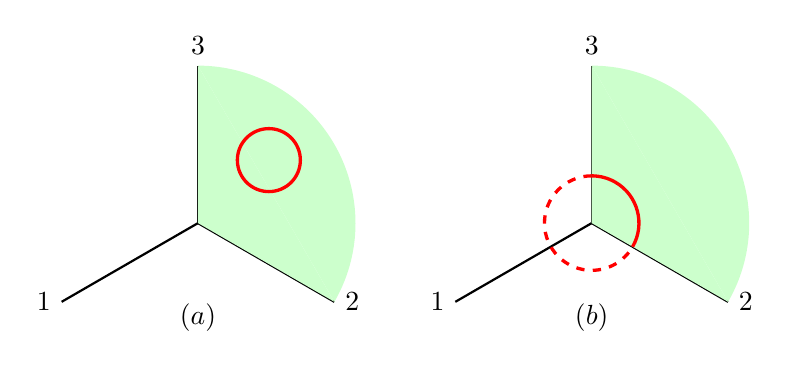
\begin{tikzpicture}

  % coordinates for the rectangle
  \coordinate (O1) at (0, 0);
  \coordinate (O2) at ($(O1) + (5, 0)$);
  \coordinate (O3) at ($(O2) + (5, 0)$);
  
  % draw the 1st configuration
  \draw[color=black, thick] (O1) -- ($(O1) + (0, 2)$) node[above=0.2]{3};
  \draw[color=black, thick] (O1) -- ($(O1) + (1.732, -1)$) node[right=0.2]{2};
  \draw[color=black, thick] (O1) -- ($(O1) + (-1.732, -1)$) node[left=0.2]{1};
  \fill[fill=green!20] ($(O1) + (1.732, -1)$) arc (-30:90:2);
  \fill[fill=green!20] (O1) -- ($(O1) + (1.732, -1)$) -- ($(O1) + (0, 2)$);
  \draw[color=red, very thick] ($(O1) + (0.9, 0.8)$) circle (0.4);

  \node at ($(O1) + (0, -1.2)$) {$(a)$} ;

  % draw the 2nd configuration
  \draw[color=black, thick] (O2) -- ($(O2) + (0, 2)$) node[above=0.2]{3};
  \draw[color=black, thick] (O2) -- ($(O2) + (1.732, -1)$) node[right=0.2]{2};
  \draw[color=black, thick] (O2) -- ($(O2) + (-1.732, -1)$) node[left=0.2]{1};
  \fill[fill=green!20] ($(O2) + (1.732, -1)$) arc (-30:90:2);
  \fill[fill=green!20] (O2) -- ($(O2) + (1.732, -1)$) -- ($(O2) + (0, 2)$);
  \draw[color=red, very thick] ($(O2) + (0.6*0.866,- 0.3)$) arc (-30:90:0.6);
  \draw[dashed, color=red, very thick] ($(O2) + (0, 0.6)$) arc (90:330:0.6);

  \node at ($(O2) + (0, -1.2)$) {$(b)$} ;

  % % draw the 3rd configuration
  % \draw[color=black, thick] (O3) -- ($(O3) + (0, 2)$) node[above=0.2]{3};
  % \draw[color=black, thick] (O3) -- ($(O3) + (1.732, -1)$) node[right=0.2]{2};
  % \draw[color=black, thick] (O3) -- ($(O3) + (-1.732, -1)$) node[left=0.2]{1};
  % \fill[fill=green!20] ($(O3) + (1.732, -1)$) arc (-30:90:2);
  % \fill[fill=green!20] (O3) -- ($(O3) + (1.732, -1)$) -- ($(O3) + (0, 2)$);
  % \draw[color=red, very thick, big arrow=<] ($(O3) + (0.6*0.866,- 0.3)$) arc (-30:90:0.6);
  % \draw[dashed, color=red, very thick] ($(O3) + (0, 0.6)$) arc (90:330:0.6);

  % \node at ($(O3) + (0, -1.2)$) {$(c)$} ;


\end{tikzpicture}
\endpgfgraphicnamed

\end{document}